\documentclass{article}

\usepackage{cite}
\usepackage{float}
\usepackage{bibcheck}
\usepackage{graphicx}
\usepackage[justification=centering]{caption}
\usepackage{amssymb}
\usepackage{amsopn}
\usepackage{amstext}
\usepackage{lscape}
\usepackage[justification=centering]{subcaption}
\usepackage{multirow}
\usepackage{color}
\usepackage[backref]{hyperref}

\captionsetup{compatibility=false}
\captionsetup{font={scriptsize}}
\newcommand{\reffig}[1]{Figure \ref{#1}}
\newcommand{\reftab}[1]{Table \ref{#1}}
\newcommand{\refsec}[1]{Section \ref{#1}}
\newcommand{\refequ}[1]{Equation \ref{#1}}
\newcommand{\tabincell}[2]{\begin{tabular}{@{}#1@{}}#2\end{tabular}}

\providecommand{\keywords}[1]
{
	\small	
	\textbf{\textit{Keywords---}} #1
}

\title{A Novel Approach of Medical Concept Mapping via Syntax-Semantics-Pragmatics Levels}
\author{Internship Candidate: Shuyue Jia}

\begin{document}
\maketitle

\begin{abstract}
Towards building an Artificial Intelligence-oriented (AI) healthcare system, precise mapping of medical concepts is highly demanded. Traditional works decoded medical terms lacking the consideration of a comprehensive overview of Natural Language Processing (NLP). However, for downstream NLP tasks, an analysis from different perspectives grows popular. In this work, a novel approach of medical concept mapping was presented from three aspects of NLP analysis, i.e., syntax, semantics, and pragmatics levels. Via the Byte Pair Encoding (BPE) Algorithm, the subwords' representations were introduced to learn the compounding and transliteration of medical concepts. Then, knowledge graph took advantages of human common sense in the perspective of pragmatics analysis. The final pre-trained word embedding and cosine similarity were utilized to map the input to the standard term which retain the maximum similarity. From the above three levels, the proposed approach has achieved compelling performance in the Chinese medical dataset, 96.81\% accuracy. It indicated that our proposed method was able to handle the challenge of medical concept mapping, which can indirectly promoted the performance of healthcare AI systems.
\end{abstract}

\keywords{Healthcare System, Artificial Intelligence (AI), Medical Concept Mapping, Byte Pair Encoding (BPE), Knowledge Graph, Word2vec}

\section{Introduction}
These days, Artificial Intelligence (AI) gains popularity and its applications have walked into people's daily life, e.g., smart home, health AI system, self-driving cars, and etc. Among all the applied fileds, healthcare is paid a lot of attention because of vast profitable markets and governments' development plans (e.g., China’s New Infrastructure Plan). In the enterprise-level healthcare AI system, taking IBM Watson Medical AI module as an example, an NLP engine was widely presented including data pre-processing, Natural Language Processing (NLP) downstream tasks (Concept Mapping, Named Entity Recognition (NER), Relation Extraction (RE)) to query-parser or other related applications. Multiple modules must be coordinated and worked smoothly to ensure the highest standards of quality and the best user experience. However, during the model establishment, errors were accumulated, which intrinsically weaken the performance of the overall system. As a result, the researchers and engineers designed and deployed each module dedicatedly and seriously. As a beginner of the NLP engine, Medical Concept Mapping was broadly studied and applied, which in some sense critical and essential to the followed modules. Traditional methods mostly utilized rule-based look-up directory to map the non-standard terms to expert-defined standard medical terms. However, it can be time-consuming and labor-intensive. Thus, in this paper, we introduced a novel method which considered all the aspects of NLP analysis, i.e., syntax, semantics, and pragmatics levels. It intended to build a robust and fast medical concept mapping model for enterprise-level NLP engine to reduce module error accumulation and enhance system efficiency.

\section{Method}
\subsection{Subwords via BPE Algorithm}
\subsubsection{Data Pre-processing}\label{Pre-processing}
In this work, we focused on the concept mapping for Chinese medical terms. First of all, all the punctuations were removed from the dataset and the input non-standard terms. Then, English and numbers in the terms were also stripped and the continuous English and numbers were put into the subwords list. Next, we deleted all the duplicated terms in the dataset to eliminate repeated terms' interference and distinguish different medical terms. The pre-processed data was utilized to obtain the most frequently appeared subwords via the Byte Pair Encoding (BPE) Algorithm\cite{gage1994new}.

\subsubsection{Byte Pair Encoding Algorithm}\label{BPE}
The BPE Algorithm was first proposed by Philip \emph{et al.} to compress data. It replaced the most common pair bytes with a new byte that did not occur in the data. When applied in the NLP tasks, it has shown that the algorithm can learn the compounding and transliteration information from subwords' representations, and generalize to translate and produce new words that were unseen at the training time. At present, the BPE algorithm was widely applied for NLP downstream tasks, like Neural Machine Translation (NMT)\cite{sennrich2015neural}, and it was also employed in the NLP pre-trained models, like Google BERT\cite{devlin2018bert} and OpenAI GPT-3\cite{brown2020language}.

The motivation applying the BPE algorithm is that in the medical field, a Chinese medical term often consists of several subwords, and they can in return interpret original word. In this work, we implemented the algorithm to large amount of medical term datasets and obtained the most frequently used Chinese medical subwords. To get subwords, the implementation details were shown below.

\textbf{1}. Initialize word vocabulary as characters, where each two characters were separated by a space. 

\textbf{2}. Summary the most frequent two-gram pairs (‘A’, ‘B’) from all the terms.

\textbf{3}. Merge (‘A’, ‘B’) → (‘AB’) and repeat \textbf{2}.

\textbf{4}. Stop merging until reaching the number of merge operations or minimum frequency.

After the above process, the most frequently appeared pairs and their occurred frequency were obtained. The pairs will be utilized to get the subwords of the input term. 

\subsubsection{Forward and Backward Maximum Matching Algorithm}\label{FMM-BMM}
To get the subwords of a concept term, based on the obtained subwords list $S$, the Forward Maximum Matching (FMM) and Backward Maximum Matching (BMM) Algorithms were implemented. Taking the maximum length $\emph{l}$ of the subword in the subwords list, the FMM or BMM algorithm sweep length $\emph{l}$'s characters $C_l$ in the input term and match it into the subword list. If $C_l$ in the subwords list $S$, then $C_l$ will be a subword of this input term. Then skip $C_l$ and continue to match. If  $C_l$ is not in subwords list, the length $\emph{l}$ will decrease by one and continue to match. The FMM matched maximum characters from left to right and BMM was reversed. After matched all the subwords, the repeated ones were removed. The left unrepeated subwords would be the subwords of the input term.

\subsection{Knowledge Graph}\label{Knowledge-Graph}
An expert pre-defined Knowledge Graph was utilized to gain human knowledge and common sense. The standard and synonym concepts were used in this work. The synonym terms were the synonyms of the standard concepts. The synonyms were connected to the standard terms as a reference of concept mapping. An example can be seen in \reffig{Standard-Synonym-Terms}. In this work, after obtained the subwords of the input non-standard term, we mapped each subword to standard or synonym terms according to the knowledge graph. If there was a mapping, the standard term was then used as matched standard term. Otherwise, it would not be used.

\begin{figure}[h]
	\centering
	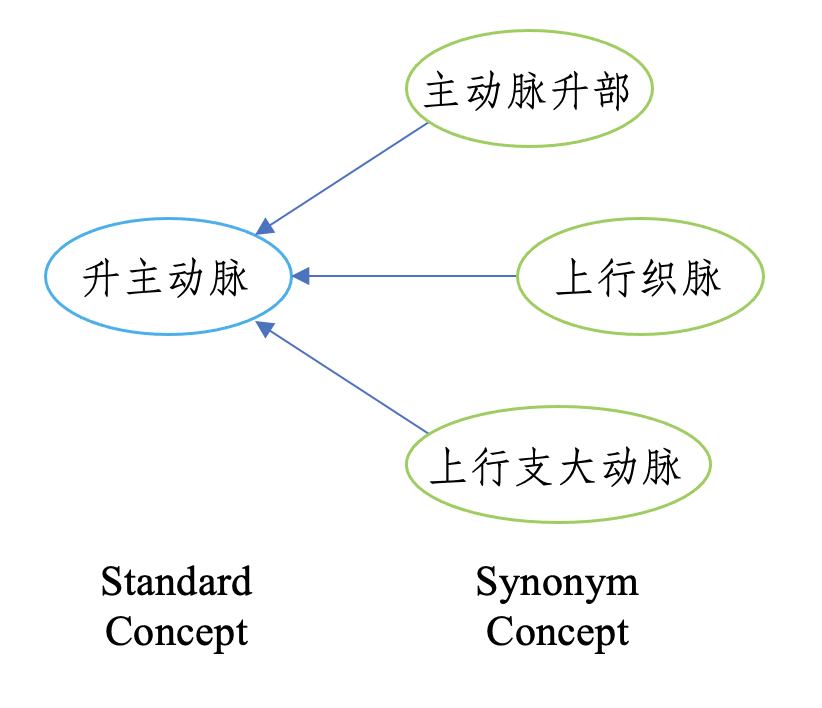
\includegraphics[width=2in]{Standard-Synonym-Terms.png}
	\caption{An example of standard and synonym terms (concepts).}
	\label{Standard-Synonym-Terms}
\end{figure}

\subsection{Word Embedding and Similarity}
In this work, we employed word2vec Skip-gram model\cite{mikolov2013efficient} to obtain the semantics information of the Chinese medical terms. During the process, there are no direct embedding for lots of terms. Thus, we use the mean of subwords' embedding for the standard terms, and the mean of matched standard terms in \refsec{Knowledge-Graph}, Jieba tokens and subwords of the input term. To measure the embeddings, we utilized cosine similarity as shown in \refequ{cosine}.

\begin{equation}\label{cosine}
	cos(\theta)=\frac{A\cdot B}{||A||\times||B||}
\end{equation}

In \refequ{cosine}, $cos(\theta)$ is the cosine similarity between the standard term $A$ and the input term $B$. We implemented Matrix Multiplication for input term $B$ with all the standard terms and return the most similar term as the final mapped standard term.

\subsection{Model Architecture}
The presented model consists of three parts, i.e., syntax level, semantics level, and pragmatics level. The system framework displays in \reffig{method}.


\begin{figure}[h]
	\centering
	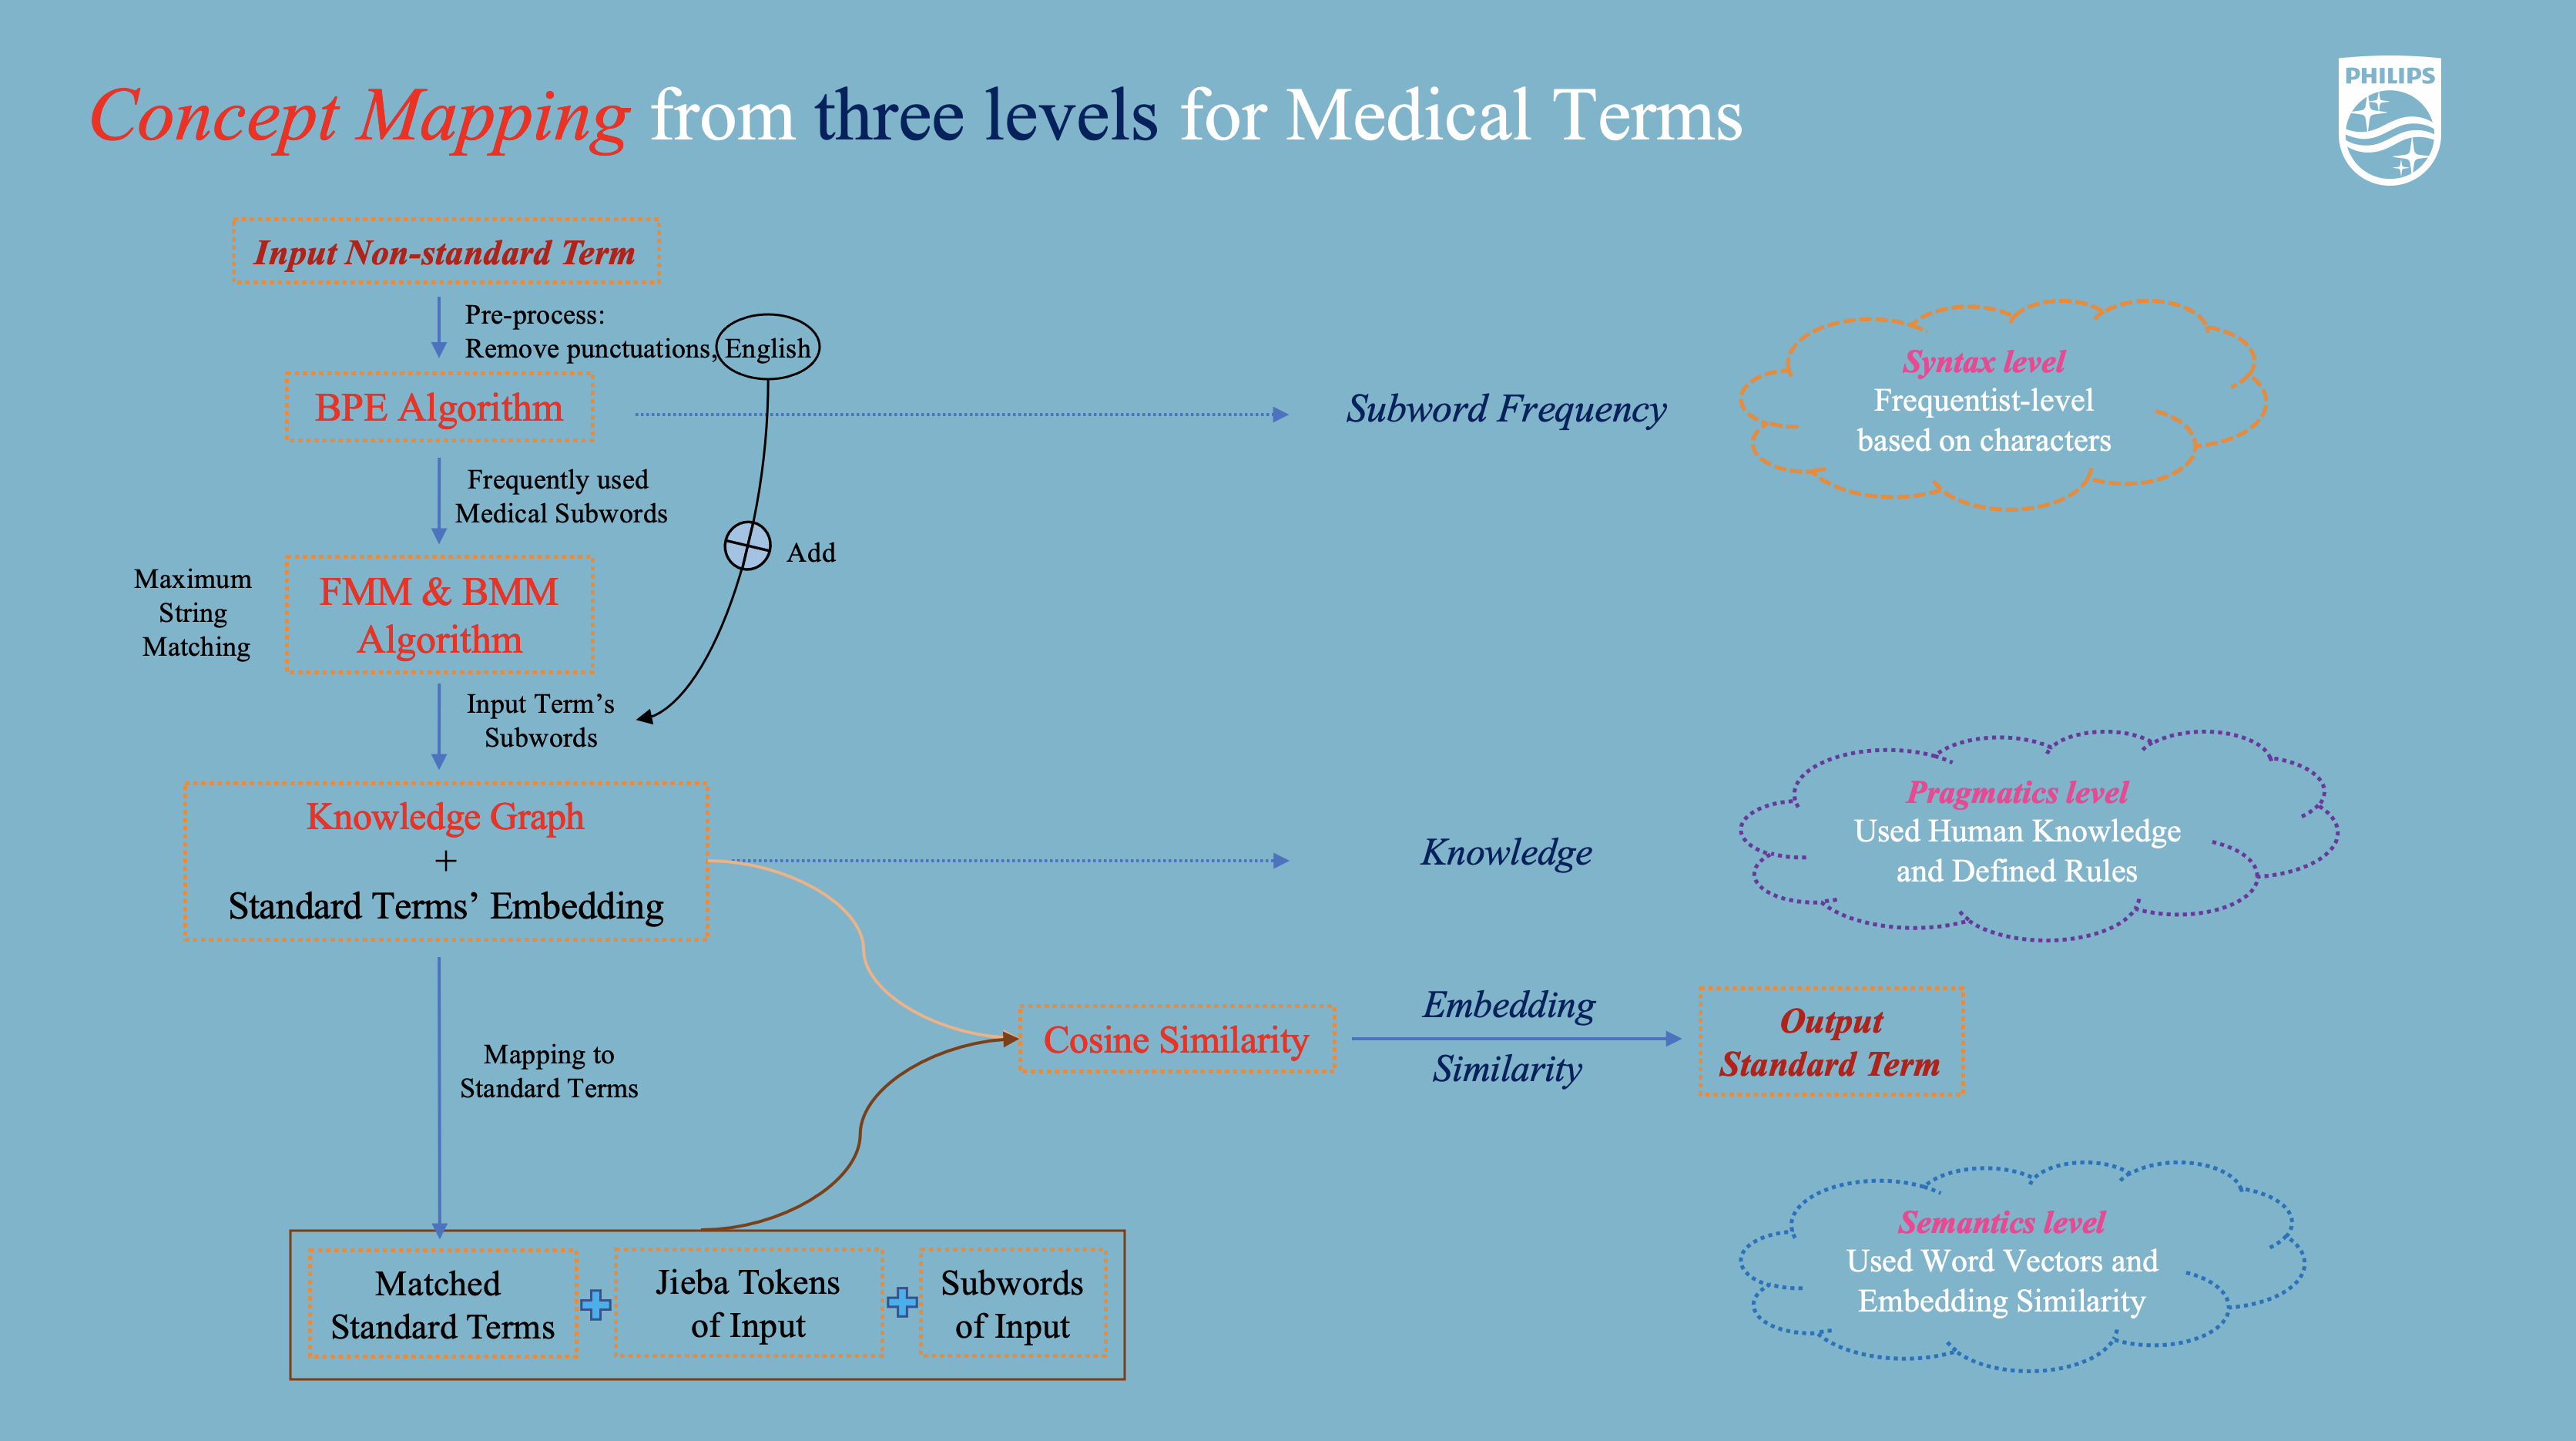
\includegraphics[width=\linewidth]{method.png}
	\caption{The system framework including syntax, semantics, and pragmatics levels for Medical Concept Mapping.}
	\label{method}
\end{figure}

The input of the presented model is the non-standard term. It has been pre-processed as demonstrated in \refsec{Pre-processing}. Then, in the perspective of syntax-level analysis, the BPE Algorithm was implemented to obtain frequently used medical subwords in \refsec{BPE}. Next, the FMM and BMM Algorithm were employed to get the subwords of the input term in \refsec{FMM-BMM}. As illustrated in \refsec{Knowledge-Graph}, from the knowledge graph (an Pragmatics level analysis), we can obtain the matched standard term with regard to each subword. Finally, based on the semantics-level analysis, using cosine similarity, the input non-standard term was mapped to the standard concept.

\section{Numerical Experiments}
\subsection{Dataset Description}
The dataset was the Knowledge Graph Dataset at Philips Research. As discussed in \refsec{Knowledge-Graph}, standard and synonym terms were applied to evaluate the introduced framework.

\subsection{Model Evaluation}
In this paper, we evaluated the performance of our model using accuracy. The accuracy of our model was 96.81\%. The result was promising that from three levels of NLP analysis, i.e., syntax, semantics, and pragmatics, the non-standard term can be correctly mapped to standard concept.

\section{Conclusion}
In this work, we applied the idea of different aspects of NLP analysis including syntax, semantics, and pragmatics to handle the medical concept mapping challenge. At the syntax level, concepts' subwords and their frequencies were investigated to learn the compounding and transliteration of medical terms, which interprets concepts' meaning. Then, knowledge graph was put forward to add human knowledge and common sense to the system as a pragmatics level analysis. Finally, at the semantics level, word2vec and cosine were used to measure the similarity between input term and standard concepts. The performance of this three-level framework was competitive and effective. The method can be employed as a part of the NLP engine to build a robust medical AI system. 

\bibliographystyle{unsrt}
\bibliography{bibliography}
\end{document}